\documentclass[table, 12pt]{article}
\usepackage{graphicx}
\usepackage[T1]{fontenc}
\usepackage{tocloft}
\usepackage{todonotes}
\usepackage{caption}
\usepackage{hyperref}
\usepackage{booktabs}
\usepackage{listings}
\usepackage{pdfpages}
\usepackage{pdflscape}
\usepackage{textpos}
\usepackage{scrhack}
\usepackage{xcolor}
\usepackage{float}
\usepackage{longtable}
\usepackage{enumerate}
\usepackage{tasks}
\usepackage{tabularx}
\usepackage{titlesec}
\usepackage{listing}
\usepackage{graphicx}
\usepackage{subcaption}

\hyphenation{group-ed}

\titleformat{\paragraph}
{\normalfont\normalsize\bfseries}{\theparagraph}{1em}{}
\titlespacing*{\paragraph}
{0pt}{3.25ex plus 1ex minus .2ex}{1.5ex plus .2ex}
\begin{document}
\begin{titlepage}
    \centering
    {\scshape\large AY 2021/2022 \par}
    \vfill
    
\includegraphics[width=100pt]{assets/logo-polimi-new}\par\vspace{1cm}
    {\scshape\LARGE Politecnico di Milano \par}
    \vspace{1.5cm}
    {\huge\bfseries Acceptance Testing Document \par}
    \vspace{2cm}
    {\Large {Ottavia Belotti\quad Alessio Braccini\quad Riccardo Izzo}\par}
    \vfill
    {\large Professor\par
        Elisabetta \textsc{Di Nitto}}
    \vfill
    {\large \textbf{Version 1.0} \\ \today \par}
\end{titlepage}
\hypersetup{%
    pdfborder = {0 0 0}
}
\thispagestyle{plain}
\pagenumbering{gobble}
\mbox{}
\newpage
\pagenumbering{roman}
\tableofcontents
\newpage
\pagenumbering{arabic}

\section{Tested Project}
\begin{itemize}
    \item \textbf{Authors}\\Valerio De Luca\\Giovanni De Novellis\\Sairaghav Venkataraman
    \item \textbf{Repository URL}\\ \underline{\url{https://github.com/sairaghav/DeLucaDeNovellisVenkataraman}}
    \item \textbf{Documents considered}\begin{itemize}
              \item RASD: Requirements Analysis Specification Document;
              \item DD: Design Document;
              \item ITD: Implementation and Testing Document;
          \end{itemize}
\end{itemize}
\newpage

\section{Installation}
The installation went very smoothly following the guide present in the ITD. The Docker solution required minimal effort from us to install the whole software. Moreover, the database dump included within the Docker sped up even more the process, since it allowed us to not create another database and make up some new entries to try the WebApp out.

\section{Acceptance Test Cases}

\subsection{Sign up \& Log in}
\begin{itemize}
    \item[\textit{i.}] \textbf{Goal} User authentication
    \item[\textit{ii.}] \textbf{Test Cases}
    \begin{itemize}
        \item[(a)] Create a new user.
        \item[(b)] Login with existing user.
        \item[(c)] Login with incorrect password.
    \end{itemize} 
    \item[\textit{iii.}] \textbf{Test Results}
    \begin{itemize}
        \item[(a)] After filling all the required fields, the user is successfully created.
        \item[(b)] Using an email and password for an existing user, we manage to succesfully log into the application and be redirected toward the user's specific homepage.
        \item[(c)] When trying to login with an existing user but an incorrect password, the access is rejected as expected, however the application gives an incorrect error message: "User with this email already exists". 
    \end{itemize} 
    \item[\textit{iv.}] \textbf{Issues}    
    \begin{itemize}
        \item The error messages are not really taken care as one would expect, since they're not always coherent with the error itself. For test \emph{(c)}, the error message is misleading, since it made us doubt that the registration phase of the new user went wrong, but instead we were just typing the password incorrectly.
    \end{itemize} 
\end{itemize}
\subsection{Dashboard}
\begin{itemize}
    \item[\textit{i.}] \textbf{Goal} Visualize regional weather conditions' data
    \item[\textit{ii.}] \textbf{Test Cases}
    \begin{itemize}
        \item[(a)] Retrieved and visualized data from 01/01/2021 and 31/03/2021 (valid date for which we knew there were data in the backend).
        \item[(b)] Tried to retrieve data for future dates.
    \end{itemize}
    \item[\textit{iii.}] \textbf{Test Results}
    \begin{itemize}
        \item[(a)] Successfully retrieved all the data.
        \item[(b)] Nothing to show. It correctly tells that there's no weather data for the specified period.  
    \end{itemize} 
    \item[\textit{iv.}] \textbf{Issues}  Nothing to highlight. Everything works fine. 
\end{itemize}

\subsection{Review Farmer Performance}
\begin{itemize}
    \item[\textit{i.}] \textbf{Goal} View information regarding best and worst performing farmers
    \item[\textit{ii.}] \textbf{Test Cases}
    \begin{itemize}
        \item[(a)] After validating a farmer's report from the agronomist user, we checked the date range and retrieved the farmer performance from agronomist user.
    \end{itemize}
    \item[\textit{iii.}] \textbf{Test Results}
    \begin{itemize}
        \item[(a)] Entry about farmer is presented to the policy maker successfully: the efficiency is calculated, the farmer can be awarded as well. The list of best and worst farmers is correctly presented in ascending and descending order respectively.
    \end{itemize} 
    \item[\textit{iv.}] \textbf{Issues}
    \begin{itemize}
        \item Search function doesn't work very well, since a report validated today can only be taken into consideration in computing the efficiency if the search is performed specifying as upperbound the date of tomorrow, which is not very intuitive.
    \end{itemize} 
\end{itemize}

\subsection{Review Agronomist Performance}
\begin{itemize}
    \item[\textit{i.}] \textbf{Goal} View information regarding best and worst performing agronomist
    \item[\textit{ii.}] \textbf{Test Cases} 
    \begin{itemize}
        \item[(a)] After validating 2 farmer's reports from agronomist user, retrieve list of best/worst performing agronomists from policy maker user.
    \end{itemize} 
    \item[\textit{iii.}] \textbf{Test Results}
    \begin{itemize}
        \item[(a)] Entry about agronomist is presented to the policy maker successfully: the efficiency is calculated. The list of best and worst agronomist is correctly presented in ascending and descending order respectively.
    \end{itemize} 
    \item[\textit{iv.}] \textbf{Issues}
    \begin{itemize}
        \item Search function doesn't work very well, since a report validated today can only be taken into consideration in computing the efficiency if the search is performed specifying as upperbound the date of tomorrow, which is not very intuitive.
    \end{itemize} 
\end{itemize}

\subsection{Visit Schedule Functionalities}
\begin{itemize}
    \item[\textit{i.}] \textbf{Goal} Visualize visit schedule and add/update schedules for agronomist user
    \item[\textit{ii.}] \textbf{Test Cases}
    \begin{itemize}
        \item[(a)] Create a new daily plan for 10/02/2022 adding farmers from the selection bar.
        \item[(b)] Confirm an already existing schedule. We marked as completed the daily plan for 10/02/2022 that has been created the day before.
        \item[(c)] Visualize created schedules in the monthly calendar, searching for 10/02/2022.
        \item[(d)] Using a new agronomist user created by us, search for a date.
    \end{itemize} 
    \item[\textit{iii.}] \textbf{Test Results}
    \begin{itemize}
        \item[(a)] The plan is successfully created, however it is possible to add the same farmer multiple times.
        \item[(b)] We were able to change the schedule status on 10/02/2022, swapping between "completed" and "not completed", as many time as we'd like.
        \item[(c)] The search results in showing the calendar of February 2022. In cell 10/02/2022 there is the list of farmers planned to be visited for that day. However, the view is a bit buggy (more in the \emph{Issues} section).
        \item[(d)] The WebApp crashes, probably because there are no schedules or farmers associated to that agronomist user yet. So this error has not been managed.
    \end{itemize} 
    \item[\textit{iv.}] \textbf{Issues}
    \begin{itemize}
        \item The same farmer can be added an infinite amount of times in a single schedule and it doesn't make sense.
        \item The visualization feature via monthly calendar doesn't practically work when an agronomist plans to visit more than 1 farm in a day, since the calendar cell is too small to fit more than that. This results in the list of added farmers to roll down behind the calendar and eventually pop up again where the latter is over. See \emph{fig. \ref{fig: calendar_bug}} for reference.
        \item It doesn't really make sense that the visualization of reports is filtered by the exact date, but then the whole month is shown. 
    \end{itemize} 
\end{itemize}
\begin{figure}[H]
    \centering
    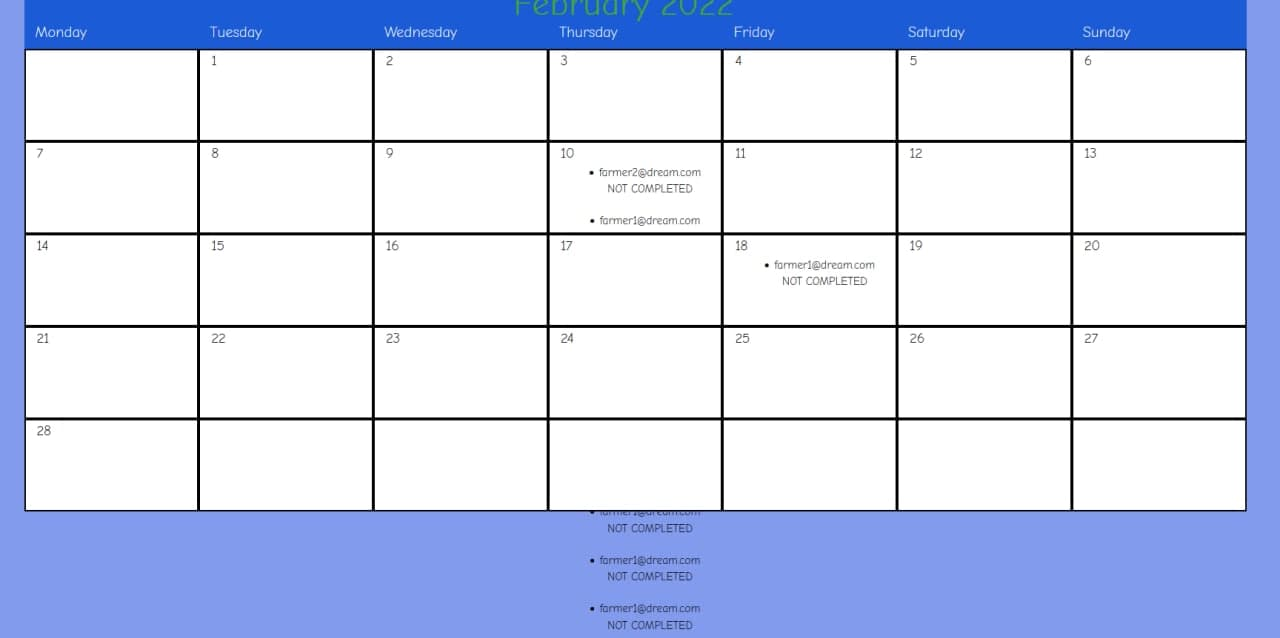
\includegraphics[scale=1.2]{assets/calendar_bug.jpg}
    \caption{Calendar view bug: many farmers scheduled for a day}
    \label{fig: calendar_bug}
\end{figure}

\subsection{Report Functionalities}
\begin{itemize}
    \item[\textit{i.}] \textbf{Goal} Visualize and review farmers' report for agronomist user
    \item[\textit{ii.}] \textbf{Test Cases}
    \begin{itemize}
        \item[(a)] Visualize report queue
        \item[(b)] Report's approval
        \item[(c)] Report's rejection 
    \end{itemize} 
    \item[\textit{iii.}] \textbf{Test Results}
    \begin{itemize}
        \item[(a)] Queue works fine, showing all the reports yet to be evaluated by the agronomist.
        \item[(b)] Once we've filled the requested fields on a report and clicked on "Approve" button, it succesfully disappears from the agronomist reports queue and the associated policy maker user can see the approved reports in the Review Agronomist section.
        \item[(c)] Once we've filled the requested fields on a report and clicked on "Reject" button, it succesfully disappears from the agronomist reports queue and the associated policy maker user can see the rejected reports in the Review Agronomist section.
    \end{itemize} 
    \item[\textit{iv.}] \textbf{Issues} 
    \begin{itemize}
        \item Filling all the required fields, mostly the "best practices used" and "practices to be avoided" fields, is difficult because it's not likely that an agronomist can grasp what best and worst practices have been used by only referring to the data included in the report by the farmer (reference \emph{fig. \ref{fig: report_review}}).
        \item After the approval or rejection of a report, the webapp doesn't root back to the Home or even Report Queue, instead it stays on the specific report page as if something didn't work. Only a message at the bottom tells us that the report has been reviewed successfully. 
    \end{itemize}   
\end{itemize}
\begin{figure}[H]
    \centering
    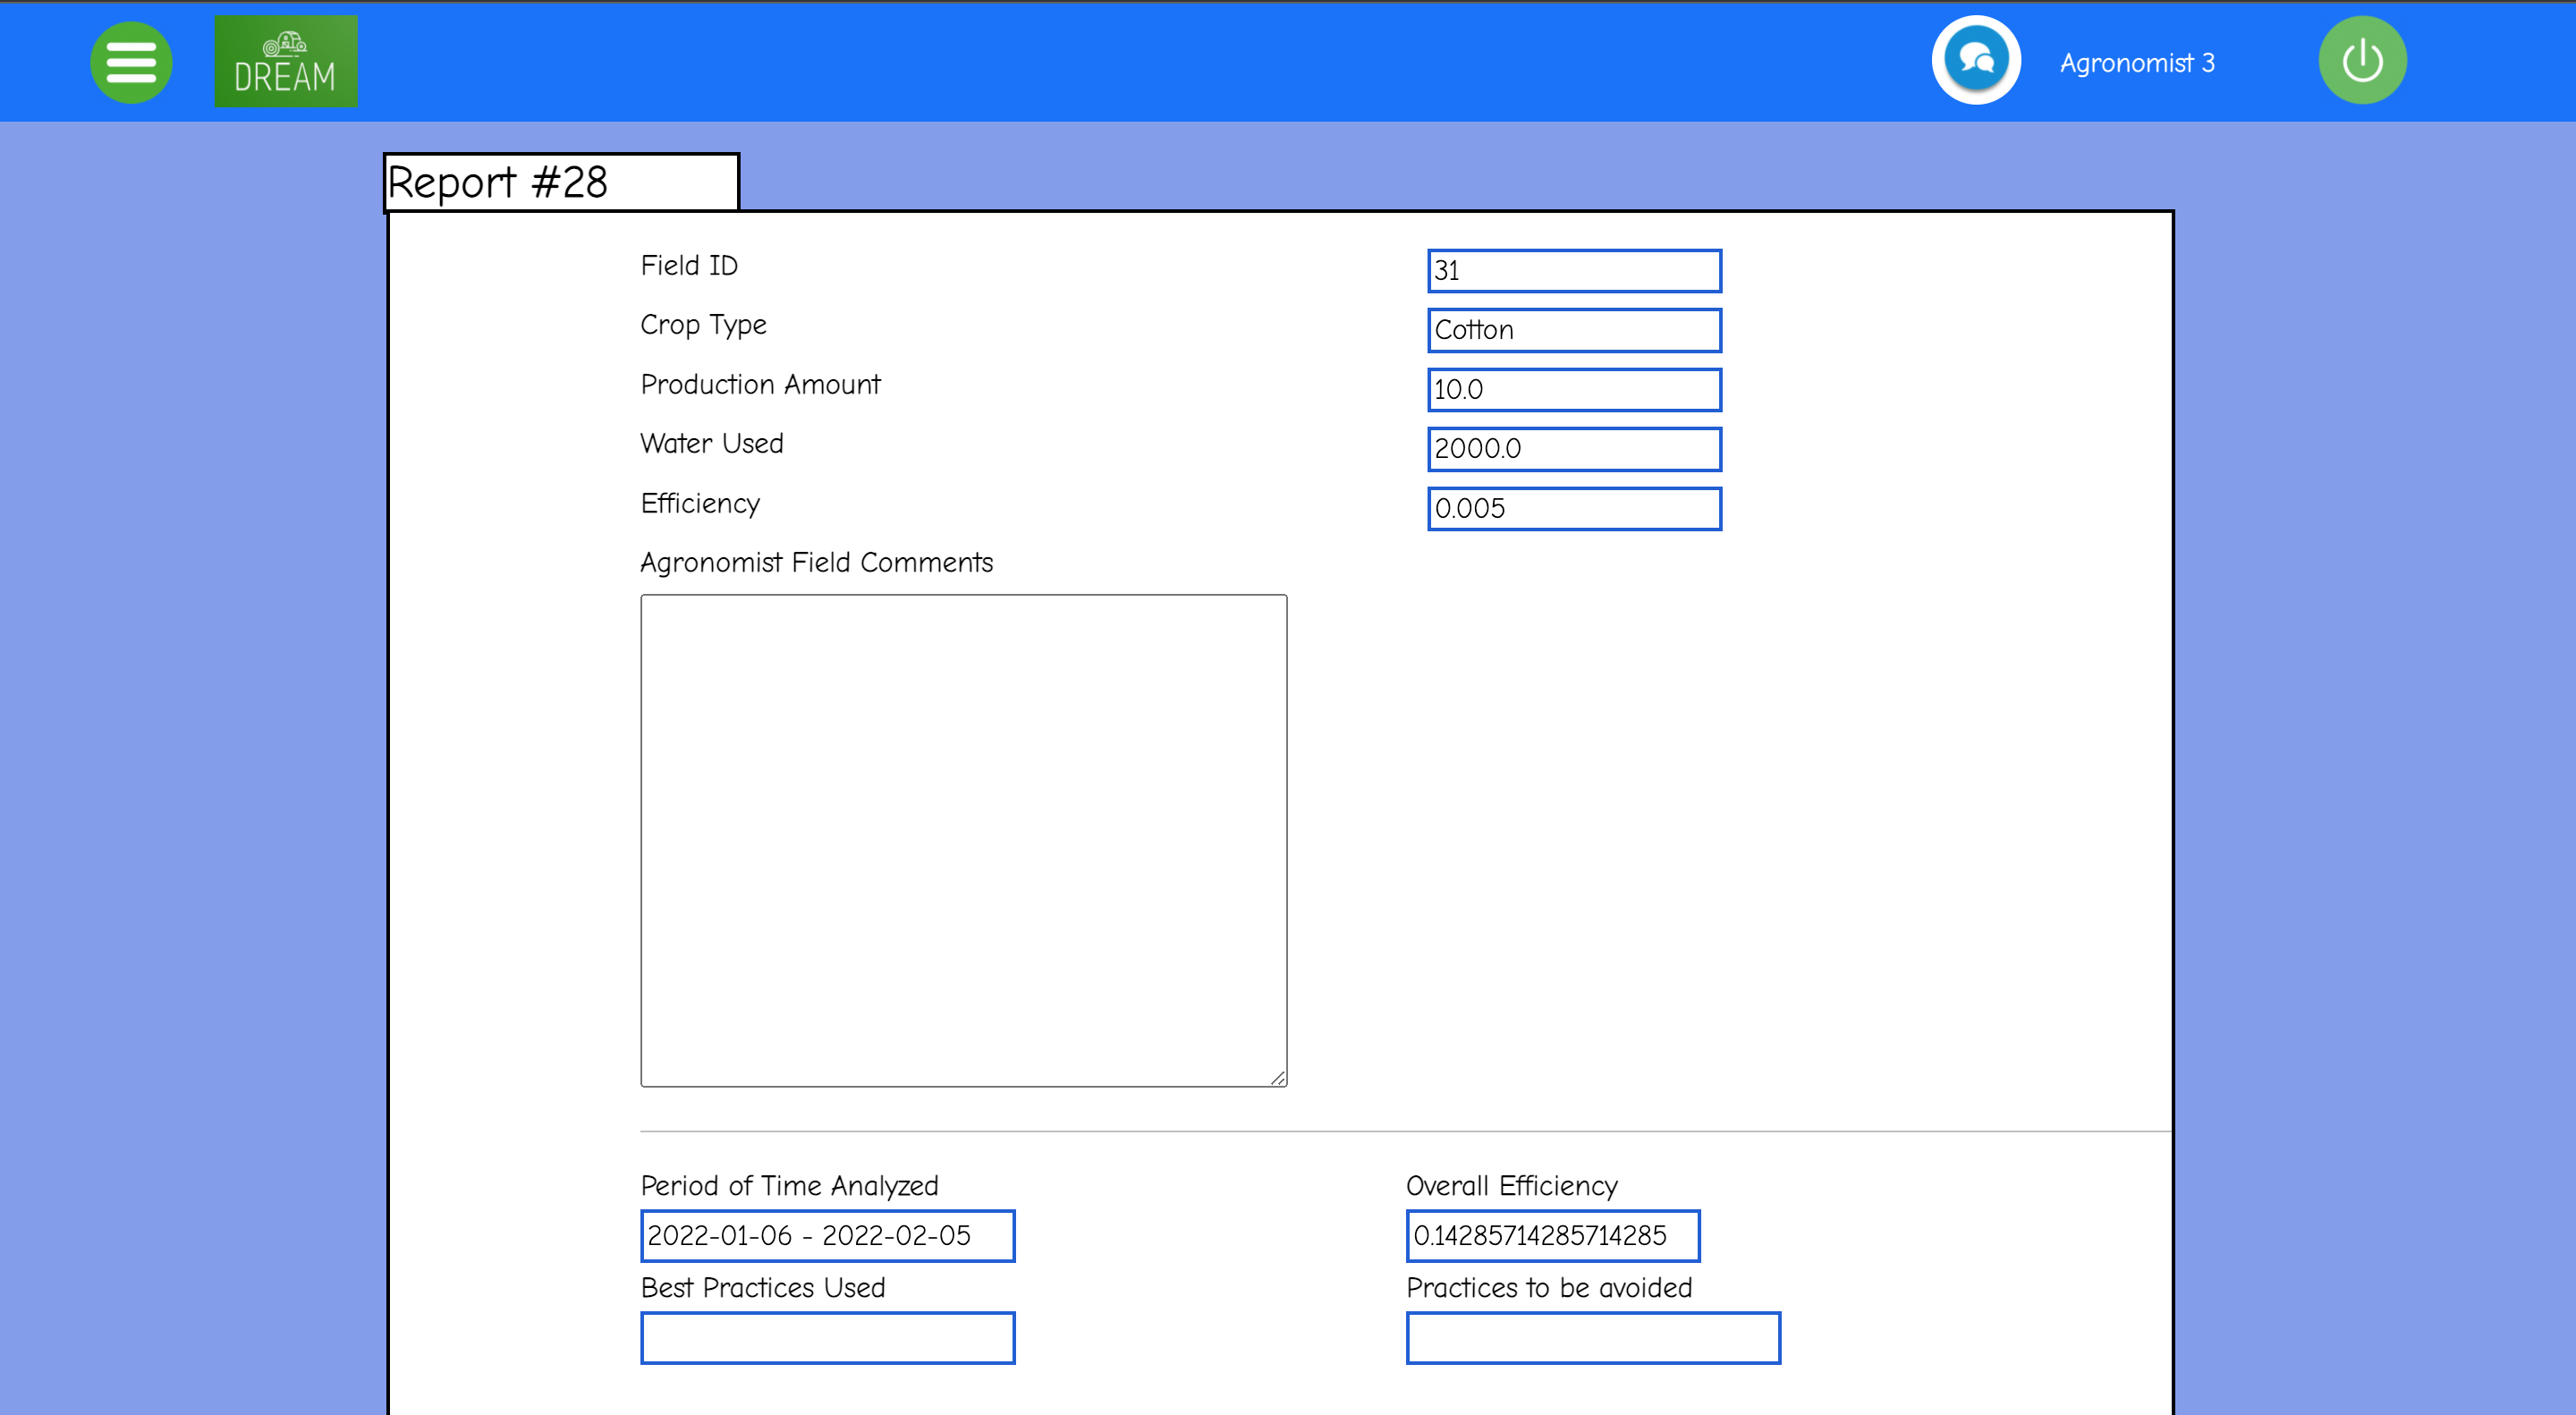
\includegraphics[scale=0.3]{assets/report_review.png}
    \caption{Report review format}
    \label{fig: report_review}
\end{figure}


\section{Project Inspection}

\subsection{Document Quality}
\subsubsection{RASD}
The RASD is well written, it is full of meaningful and detailed graphs as state diagrams, use-case diagrams and sequence diagrams. 

Moreover, in general it isn't too technical, as this type of document requires since it is meant to be read by different type of stakeholders, even without any IT background.

However, the steering initiatives aspect required by the specification is not even mentioned, neither a functionality for the policy makers to review them is implemented.

Overall, we think the RASD is very well done.

\subsubsection{DD}
The general Application Server Component diagram presents all the manager components as black boxes, that are further developed later, one by one. Because of this approach, the interfaces between subcomponents are not very clear. Also, the specific \emph{Performance Manager}'s diagram is not coherent with the main component diagram, because it is said to communicate with the \textit{Request Router} instead of the DBMS (\textit{AccessDB}).
Overall though, the presented components are enough and it seems like nothing crucial is missing, they are also thoroughly described as well.

Finally, there are a lot of useful mockups to visualize the preview of the WebApp.

\paragraph{Testing}
The testing plan is detailed since there are specified all the Manager components to be tested and  which kind of test to perform on them, however, since they deeply specified them, we can say that they didn't take a lot of possible corner-case tests into consideration. Comparing the test plan with the actual testing in the development phase, it seems that the group has focused on testing mostly correct behaviours, but has not checked that unwanted ones don't occur as well. 

\subsubsection{ITD}
The ITD extensively explains the implemented functionalities, but the users' description reminds us that agronomists and policy makers should be able to send messages to each other directly in-app even though the chat feature is not implemented.

The frameworks choice has been a bit superficially motivated.

The installation section is very well done: the guide is clear and the fact that a Docker container has been provided makes it very easy to install the software and start the server.

\subsection{Architecture Quality}
The architecture is 3-tier as stated in the DD: client, server (frontend and backend) and database. We believe it's a reasonable and standard choice.

MongoDB is also a well renowned NoSQL database system with high availability, so there's no doubt on its performance in serving the software.

\subsection{Code Quality}
The software has been written in Python using Django Framework to develop both backend and frontend. These two has been devided into two different Django Apps. 

To us, this doesn't seem a very maintainable choice because, for example, the backend functions providing the API for the frontend are all grouped in one python file (dreamAPI/view.py). In our opinion, it would have been better to divide all the backend functionalities in more Django Apps, so that every feature can have, at least, its own view.py (for the API functions) and model.py (for the database ORM) files, making the structure more modular and easier to mantain.

The code is well commented in the managers files (dreamAPI/services/*.py).

\paragraph{Testing}
The system has been tested (24 test cases present in total) and all the tests are brought out succesfully. However, they don't really test corner cases, since it seems that only the regular workflow has been checked (e.g. saving and retrieving data when the requests are mostly locially well formed), but without testing any exception that the code might raise. The crashing error found in the schedule functionality is an example that proves this point.

\section{Conclusion}
Overall, the developed software is functional, however it's not a great user experience because some design choices are not intuitive and at times complex, for instance the fact that everything is filtered by date is a bit of a hassle. Most of the time, the relevant periods would be "today", "last week", "last month" and so on; so we think it would be easier as a user to choose a pre-set period among those cited ones or consider the entire historical data of the database (in case of review farmer/agronomist performance) by default, while making the custom "filter-by-date" a secondary feature, since it would be likely less used and it's more time consuming. 



\section{Effort Spent}
\begin{tabular}{|c||c|}
    \hline
    Student & Time for acceptance testing\\ \hline
    Ottavia Belotti & 8h \\
    Alessio Braccini & 8h\\
    Riccardo Izzo & 8h \\
    \hline
\end{tabular}

\end{document}